%------------------------------------------------------------
% 3.6 Energía potencial gravitacional y electrostática de dos partículas
%------------------------------------------------------------
\subsection*{3.6 \textcolor{Cinnabar}{\textbf{Energía potencial del sistema de dos partículas:}}}

Supongamos que en el espacio se tienen dos partículas con masa y carga, ubicadas en posiciones
\(\vec{r}_1\) y \(\vec{r}_2\). La partícula 1 tiene masa \(m_1\) y carga \(q_1\); 
la partícula 2 tiene masa \(m_2\) y carga \(q_2\).
Aplicamos la \textbf{ley de gravitación universal de Newton} y la \textbf{ley de Coulomb} 
para determinar la energía potencial del sistema.

\paragraph{Sistema y coordenadas.}
\begin{center}
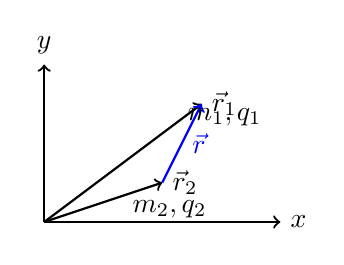
\begin{tikzpicture}[scale=1.0]
\draw[->, thick] (0,0) -- (3,0) node[right] {$x$};
\draw[->, thick] (0,0) -- (0,2) node[above] {$y$};
\draw[->, thick] (0,0) -- (2,1.5) node[right] {$\vec{r}_1$};
\draw[->, thick] (0,0) -- (1.5,0.5) node[right] {$\vec{r}_2$};
\draw[->, thick, blue] (1.5,0.5) -- (2,1.5) node[midway, right] {$\vec{r}$};
\node at (1.7,1.1) [above right] {$m_1,q_1$};
\node at (1.0,0.4) [below right] {$m_2,q_2$};
\end{tikzpicture}
\end{center}

El vector de posición relativa es
\[
\vec{r} = \vec{r}_1 - \vec{r}_2, 
\qquad 
r = |\vec{r}_1 - \vec{r}_2|.
\]

\paragraph{Fuerzas entre las partículas.}
La fuerza gravitacional es
\[
\vec{F}_g = -\,G\,\frac{m_1 m_2}{r^2}\,\hat{r},
\]
mientras que la fuerza eléctrica (de Coulomb) es
\[
\vec{F}_c = \frac{1}{4\pi\varepsilon_0}\,\frac{q_1 q_2}{r^2}\,\hat{r}.
\]

\paragraph{Potenciales asociados.}
Dado que ambas son fuerzas centrales (radiales), existe un potencial escalar \(U(r)\)
tal que \(\vec{F}=-\nabla U\). 
Integrando con respecto a \(r\):
\[
\vec{F}_g = -\,\frac{dU_g}{dr}\,\hat{r}
\quad\Rightarrow\quad
\int \frac{1}{r^2}\,dr = -\frac{1}{r} + C
\]
Por tanto, el potencial gravitacional es
\[
\boxed{U_g(r) = -\,\frac{G\,m_1 m_2}{r}}.
\]

Análogamente, para el caso eléctrico:
\[
\vec{F}_c = -\,\frac{dU_c}{dr}\,\hat{r}
\quad\Rightarrow\quad
\boxed{U_c(r) = \frac{1}{4\pi\varepsilon_0}\,\frac{q_1 q_2}{r}}.
\]

\paragraph{Energía potencial total.}
La energía potencial total del sistema de dos partículas es
\[
\boxed{U(r) = U_g + U_c = -\,\frac{G\,m_1 m_2}{r} + \frac{1}{4\pi\varepsilon_0}\frac{q_1 q_2}{r}}.
\]

\paragraph{Comentario:}
Ambos potenciales son \emph{funciones radiales inversamente proporcionales a la distancia}. 
El signo negativo en \(U_g\) refleja la naturaleza atractiva universal de la gravedad, 
mientras que el signo de \(U_c\) depende de las cargas \(q_1\) y \(q_2\), 
pudiendo representar una interacción atractiva (\(q_1q_2<0\)) o repulsiva (\(q_1q_2>0\)).
